\documentclass{article}
\usepackage{graphicx}
\usepackage{float}   
\usepackage{verbatim}
\usepackage{amsmath} 
\usepackage{amssymb} 
\usepackage{fullpage}
\usepackage{listings}
\usepackage{subfig}   
\usepackage{epsfig}
\usepackage{siunitx}
\newcommand{\quotes}[1]{``#1''}

\begin{document}

\title{MEAM520 Final Project Report}
\author{Brian Grimaldi, Venkata Gurrala, Sheil Sarda, Alexis Ward}
\date{December 2020}


\maketitle


\section{Introduction}
    %Objective/Strategies (High Level)
    %Rules that were integral to our strategy
    %Point System (Equation)

The general strategy used was to get as many dynamic and static blocks to the goal as possible. In particular, the dynamic blocks were prioritized first due to the fact that it had 3 times the number of points and were open to be taken by the other team. The dynamic blocks were stacked in a specific part of the goal position. To avoid the risk of a falling stack, the stacks for dynamic and static blocks were positioned apart at the goal platform. All the blocks in the work space can be picked up from a vertical or horizontal wrist orientation. While picking up the dynamic blocks, the horizontal wrist position was used so that we could enable a larger tolerance to grasp a block. Additionally, by using a horizontal wrist orientation, we were able to push forward upon blocks so that the orientation of the blocks aligned with the orientation of the end effector. For static blocks, a vertical orientation to pick up blocks was prioritized. By enabling the use of the rotating wrist, the end effector could easily align with the orientation of the blocks. However, not all static blocks were able to be picked up from a vertical orientation due to the fact that some blocks lied on the edge of the reachable workspace and would cause a non-feasible orientation. In this scenario, a horizontal wrist orientation was used similar to what was used when picking up dynamic blocks.

\section{Method}
    \subsection{Dynamic Blocks}
    %Sheil/Venkata
    When attempting to pick up dynamic blocks, a home position for the dynamic block picking was first defined. This is the location where the end effector is in close proximity to the rotating turn table where it is ready to position itself to approach a target block on the turn table. Figure () shows a picture of this position. As soon as the robot reaches the home position, it calculates all of the current blocks' state and determines their current angles by using the x and y position components of the transformation matrix and using the atan2 function. The angles of each block are then checked and compared in order to find the block which has smallest angle to the end effectors angle of 45 degrees from the x axis. It prioritizes the closest angle in the direction of the turntable movement. It then targets the closest block and positions the wrist such that it is 50 mm behind the block when the block is in the same plane as the robot’s wrist, as shown in figure (). The object’s state is then constantly tracked for any updated movement due to both the turn table and movement caused by opponent. When the block’s angle is within 0.05 radians of the angle of the static wrist, the robot is given the command to simply move forward in its plane. The command is given to move further forward than the block’s current position so that any difference in orientation can be fixed and the end effector can have a secure grip on the block. 
    
    \subsection{Static Blocks}
    %Venkata/Alexis
    To pick up static blocks on the platforms, the grip static and calculateIK functions were used to find the exact orientation of the robot necessary to reach a position 30 mm above the block if approach from a vertical standpoint. The grip static function prioritized the rotation of the wrist such that the orientation of the cube can be prioritized. 
    
    %need to talk more about grip static 
    \subsection{Goal Positioning}
    %Alexis/Brian
    
    \subsection{Path Planning}
    %Venkata
   The paths that the robot took throughout its run were developed to avoid collisions with the platform as well as the blocks. Since the blocks were randomlized, there would be a chance where the static or the dynamic blocks could be stacked on top of each other for the run. If the robot was not handling with blocks on a given platform, it was completely out of the vertical space of the platform to prevent knocking over stacked blocks. Rather than using path planners, a hardcoded path was developed which we determined would be more reliable since it is deterministic and would allow us to optmize for the shortest path required to move between platforms while considering the handling of the blocks between the platforms. After each dynamic block was picked up, it was taken to a preset postion on the goal platform. There were 2 intermediate commands given in the path before it went into the goal platform space. The first was the zero position and the second was the position right before entering the goal platform from a vertical position. The second intermediate command was given so that the robot's theta 1() was constant so that the arm's swinging motion would not cause any present stacks on the platform to fall over. After the last dynamic block was placed in the goal position, the robot was then tasked to move pick up the static blocks at the platform closest to the goal postion. This enabled the robot to quickly score as many points as possible, given the allotted time. Afer each static block was picked up, it slowly came out of the z axis space above the platforms before moving to the goal position to prevent any stacks on the goal from falling over. By using anywhere between 2 to 3 preset intermediate commands, we were able to eliminate the need to compute a path using a path planner such as a potential field or an RRT planner, thus saving valuable time. 
 
   
% Combine with Methods
% \section{Concepts utilized in Code}

%     \subsection{final.py}
    
    
%     \subsection{calcIK.py}
    
    
%     \subsection{gripStatic.py}


%     \subsection{Grasping}
%     %How we decide to grasp moving or static blocks.


\section{Experimental results}
%Draw upon results of the match
%Are cases chosen show advantages and disadvantages
%Brian


  
\section{Evaluation}
%Analyze the results of the match
%Brian(?)
%Blocks stacked in certain time
    %Static/Dynamics?

     \subsection{Stack Height}
		With the objective of maximizing the altitude of all the blocks on our goal platform, we decided to implement block stacking. We considered several implementation options, including tracking the position of the blocks currently on the platform and using the pose of the top most block of the stack to determine where the robot arm should drop the block. A common shortfall of this method is that if due to mechanical error, the top block is not centered on the previous block, this error will propagate up the stack, causing instability and eventually lead to a toppling over.
		
		A simpler implementation we implemented in our robot was to generate a smooth path of moving the end effector to the $X, Y$ coordinate of the center of the stack, but maintaining an altitude greater than the largest possible height of our 3-block stack. From this position, we relax the end effector and drop the block onto the tower in a controlled purely vertical motion.
	
     \subsection{Picking up Dynamic Blocks}
     
     \subsection{Wait Time for Dynamic Blocks}

     \subsection{Getting Side Bonus}


\section{Analysis}
%Conclusion
%Future work
%Strengths and weaknesses compared to other robots
The robot was able to meet the objective of getting all the blocks into goal by the 60 seconds limit in most runs. It was also able to carefully stack upto 3 blocks per stack. Some of the weakness of the robot which prevent the robot to move to the next rounds were caused by the inability to change the orientation of the blocks to keep the white face up since getting more blocks to the goal was the bigger priority. When picking up the dynamic blocks, there was time wasted waiting for the block to reach a certain angle within the turntable. This prevented the robot to make time to carefully stack more blocks and change their orientations. 


\section{Appendix}

\begin{figure}[h]
\centering
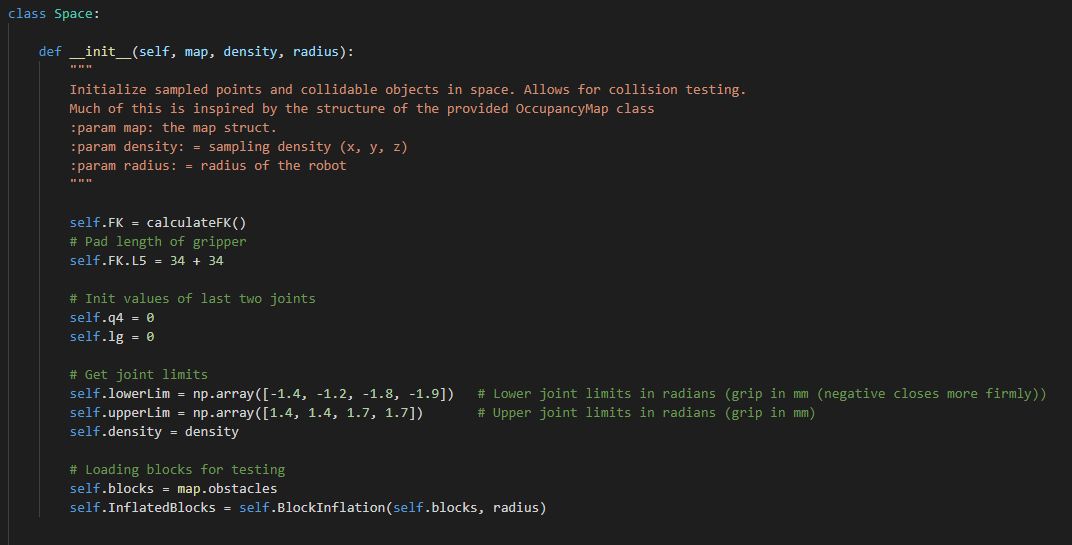
\includegraphics[scale=.6]{Fig1.png}
\caption{Initialization of Space class.  Creates a sample space object that we can call to generate random configurations (q) from.  Also inflates blocks in order to compensate for simplified representation of lynx arm geometry.}
\label{fig1}
\end{figure}


  \begin{equation}
      \gamma = \lambda* \dot{x}
  \end{equation}




\end{document}
